\documentclass[main.tex]{subfiles}

\begin{document}

\chapter{Preassembly} \label{chapter:preassembly}

Two key aspects in long-read genome assembly are 1) the detection of overlaps between reads and 2) dealing with errors in reads. Computing overlaps is done prior to assembly can thus be considered as a preassembly task, even if some assembly pipelines compute overlaps several times. Computing overlaps is a hard task, even harder with high error rate reads. A number of tools have been designed in the last decade, with their own definition of what is an 'good' overlap. The section \ref{sec:preasm:ovl} gives a short overview of algorithmic ideas on which overlappers are designed. The next section \ref{sec:preasm:blog_post} discusses about comparison of overlaps found by state-of-the-art overlappers for long read data. 

\bigskip

After sequencing a usual task is to clean the set of reads, e.g.
\begin{itemize}
	\item remove too short reads (less than 500~bp, 1000~bp or even 2000~bp)
	\item find and remove the sequencing adaptors (that is a short sequence added before DNA fragment, this short sequence is required for some biochemical consideration, but they can create trouble in assembly)
\end{itemize}
or perform some operations to improve the quality of reads, e.g.
\begin{itemize}
	\item found highly erroneous regions of reads and replace them by more correct one, this operation is called \emph{scrubbing}
	\item correct reads using information from other sequencing technology (this is called hybrid correction) or with same technology, this operation is called \emph{correction} 
\end{itemize}
Cleaning preprocessing intends to improve the quality of the assembly or to help the task of assembly (e.g. by reducing the number of false overlaps). 
As overlapping tools didn't know what the user will do with the computed set of overlaps, all information is reported (it's a good point). But one has to remember that the number of overlaps for a common sequencing experiment is very large, storing them may require more than terabyte for some large dataset. In section \ref{sec:preasm:intro_fpa} we introduce in more details this trouble and the solution we have design. \jsv{paragraphe a retravailler}

Correction and scrubbing seeks to perform the same target: reduce the error rate of reads. Scrubbing works on large region (around ten or hundred bases) while correction works at the level of one base. This difference of scale implies different requirements in terms of computation time and memory usage.

Our work on overlap selection and on scrubbing tools was merged in a paper presented in section \ref{section:preassembly:paper}.

\section{Overlaps and their impact on assembly}

\subsection{How to find similar regions between sequence} \label{sec:preasm:ovl}

As we defined in the introduction, when two sequences share a common substring, we say that they overlap or that one of them maps on the other see \ref{intro:fig:overlap:perfect}. It is possible for sequences to share a common substring just by chance (because of the 4-letter alphabet) but the probability of this event decreases when the length of the common substring increases. Intuitively, this probability gets smaller as common substring gets longer. If the reads does not contain sequencing errors, the only criteria to evaluate whether a common substring is "true" or not could be the length of this substring. However, the number of errors in the sequence of readings breaks this paradigm and forces us to integrate the errors when assessing the quality of an overlap. Figure \ref{intro:fig:overlap:erroneous} show an overlap with two mismatch. There are two base pairs that do not match between the two sequences - knowing if this overlap is "true" or not isn't obvious.


\begin{figure}[ht]
    \centering
    \subfloat[ht][$R_1$ shares 7 bases at its end with the beginning of $R_2$, without any error]{
        \subfile{introduction/tikz/perfect_overlap.tex}
        \label{intro:fig:overlap:perfect}
    }
    \subfloat[ht][$R_1$ shares 5 bases at its end with $R_3$, with one substitution and one deletion]{
        \subfile{introduction/tikz/erroneous_overlap.tex}
        \label{intro:fig:overlap:erroneous}
    }
    \caption{When reads don't contain error, overlaps look like (a), but sequencing technologies make errors and the overlap present in (b) can be a true overlap.}
    \label{intro:fig:overlap}
\end{figure}

In this document we distinguish two tasks in similarity search between two sequences:
\begin{itemize}
    \item mapping: one tries to find the position of a read in a larger sequence (e.g. comparing different datasets, experiments from different sequencing generations, or between the reads and an assembly, against a reference genome)
    \item overlapping: one tries to find which reads share a common substring with other reads (e.g. finding common substrings in the same dataset) 
\end{itemize}
Even if mapping and overlapping can be seen as different tasks, one could observe that the same tools, and underlying algorithmic, can be used to solve both tasks.


\paragraph{The seed-and-extend strategy.} 
Search of similarity between two or more DNA sequences has many links to plain text search.
Seed-and-extend is an approach used by many tools to find similar sequences between a target (e.g. a reference genome) and a query (e.g. a read). The idea is to find a high similar subsequence (often exact), namely the seed (or anchor), and then to extend this seed to have a larger common subsequence. Tools that implement this approach usually create an index of the target. This index need to answer to a simple question: is a given subsequence exist in target and at which position. Each query is processed and its substrings are searched in the index. This gives a set of seeds that can be extended through alignment techniques such as dynamic programming. If the alignment score reaches a given threshold, a hit is reported.

Many tools for mapping and overlapping use seed-and-extend strategy. The most popular is \toolsname{Blast} \cite{blast_one, blast_two}. Specific tools dedicated to sequencing are \toolsname{BWA} \cite{bwa_mem} or \toolsname{blasr} \cite{blasr}. Implementation details of indexes, size and number of anchors change between tools. For example \toolsname{BWA} or \toolsname{blasr} use a FM-index \cite{fm-index} to perform anchor search.

\paragraph{The seed-only strategy.}

With NGS technology development more and more data had to be processed and the seed-and-extend strategy was replaced by a seed-only strategy. Indeed, the extension step is still very time-consuming. With the seed-and-extend strategy, an overlap is scored by its length and the number of errors in the alignment. With the seed-only strategy we don't have an alignment. The overlap is thus scored using the number of seeds and their positions. 

This strategy was used in \toolsname{SGA} \cite{SGA} assembly tools, during overlapping step \toolsname{SGA} search exact overlap between low error read, by search a substring at end of read in a FM-index. 

Specificity of long-reads (longer reads, high error rate) has relaunched this research field. \citeauthor{ovl_bench} produce an interesting review about some of third-generation overlap search in \cite{ovl_bench}, discussed in next section. 
We can cite \toolsname{Hisea} \cite{hisea}, \toolsname{Daligner} \cite{daligner}, \mhap \cite{canu} and \minimap \cite{minimap, minimap2} as overlapping tools they use this strategy to found overlap between thrid generation overlap. We will give some details on \mhap and \minimap in section \ref{chapter:sota}.

For third generation reads, the length of the reads and the large number of errors make the choice of algorithm parameters even more complicated, particularly concerning how we choose the seed and length of seeds. But by removing the extend step the computation time was reduce and help to manage the high error rate of thrid generation reads.

\paragraph{On the importance of overlaps.}

As overlaps are the basic components to reconstruct the original sequence, a missing overlap may lead to a wrong assembly (entire pieces of the genome inverted) or to a high number of contigs. In \cite{ovl_bench}, \citeauthor{ovl_bench} compare the state of the art third generation sequencing read overlappers on simulated datasets and on real datasets. A drop in the accuracy and recall of these algorithms can be observed between real and simulated data \ref{preassembly:tab:ovl_result}.
\begin{table}[ht]
    \centering
    \begin{tabular}{l|rr|rr}
                & \multicolumn{2}{c}{Pacbio}                & \multicolumn{2}{c}{Nanopore}              \\ 
                & Simulated           & Real                & Simulated         & Real                  \\ \hline
    Sensibility & 88.9$^m$ - 92.4$^d$ & 59.6$^m$ - 83.8$^d$ & 90.4$^g$ - 95.2$^b$ & 88.9$^b$ - 92.9$^d$ \\
    Precision   & 81.9$^b$ - 96.5$^g$ & 79.8$^h$ - 96.5$^b$ & 75.1$^b$ - 99$^m$   & 73$^b$ - 95.4$^m$   \\
    \end{tabular}
    \caption{\textsuperscript{m}\toolsname{Minimap}, \textsuperscript{d}\toolsname{Daligner}, \textsuperscript{g}\toolsname{GraphMap}, \textsuperscript{b}\toolsname{BLASR}, \textsuperscript{h}\mhap}
    \label{preassembly:tab:ovl_result}
\end{table}

In a blog post "State-of-the-art long reads overlappers comparison" \footnote{\url{https://blog.pierre.marijon.fr/long-reads-overlapper-compare/}} we take the same data as \cite{ovl_bench} but we didn't care if the overlappers found 'right' or 'wrong' overlaps. Instead we searched for comparing overlaps sets to decide whether or not overlappers compute the same overlaps. There were differences large enough to justify the idea of creating a kind of 'reconciliation' tool that merge information from several overlapper. This blog post was presented at the poster session of JOBIM (\textit{Journée Ouverte de Bioinformatique \& Mathematique}) 2018.

\subfile{paper/blog_post.tex}

\newpage

\section{Improving assembly by filtering out overlaps and scrubbing}

\subsection{Improve genome assembly efficiency by reducing the quantity of information} \label{sec:preasm:intro_fpa}

Error in third generation reads make it more difficult to found overlaps between reads. Current techniques attempt to optimize results on real data \cite{ovl_bench}.
Actually, a key observation is that within the overlaps found by state-of-the-art tools, not all of them are useful to downstream analysis. For example \miniasm keeps only end-to-end overlaps, and \canu keeps only the two longest end-to-end overlaps for each read (see \ref{chapter:sota} for more details).

Figure \ref{intro:fig:length_overlap_histogram} shows a histogram of overlap lengths found by \minimap on \textit{E. coli} Nanopore dataset (acession number SRR8494940): 33 \% of overlaps are shorter than 2000 bases. By default \miniasm ignores overlaps shorter than 2000 bases that is if we run a basic \miniasm pipeline, 33\% of the overlap will not be used but they are written on the disk.  
\begin{figure}
    \centering
    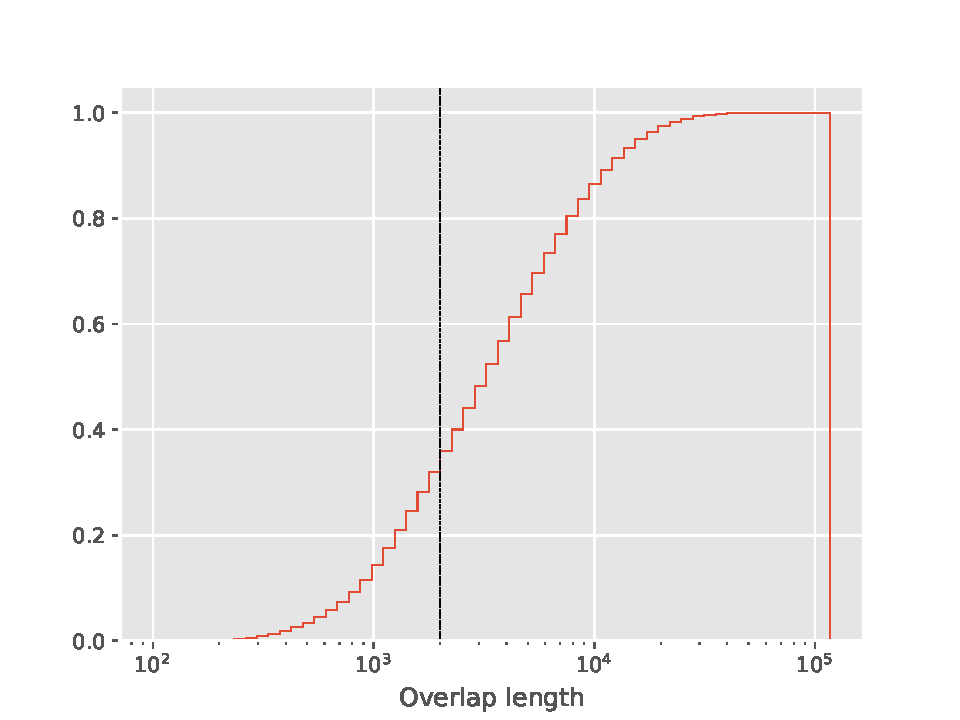
\includegraphics[width=\textwidth]{introduction/images/overlap_length.pdf}
    \caption{Histogram of overlap lengths found by \minimap, the black line represents the \miniasm overlap length threshold. The fasta file weight 3.1 Go, complete PAF file generate by \minimap weight 5.5 Go, without overlap lower than 2000 bases the weight is reduced to 3.7 Go.}
    \label{intro:fig:length_overlap_histogram}
\end{figure}
There is definitively room for improvement. Can we filter overlapping information with positive (or at least no negative) impact on assembly results ? One may hope to at least decrease the disk space and may be to increase the speed of assembly.

In section \ref{section:preassembly:paper} we present \fpa (for Filter Pairwise Alignment), our solution to filter out useless overlaps. An overlaper output can be piped directly to \fpa. \fpa can apply several filters based on length of read, length of overlap, type of overlap, read name. Some simple \fpa filters reduce the computation time of assembly without effect (or a small positive effect) on assembly.


\subsection{Read scrubbing: an alternative to read correction} \label{sec:preasm:intro_yacrd}

Assembly tools are based on reads. If your reads are bad, your assembly will be bad. To continue on the analogy given in the introduction, you probably cannot reconstruct a book if crazy monks gave you only fragments with half of the letters being erroneous. Correction of reads, with a mix of sequencing technologies or with a single technology, can help to get better reads. But actually, correction tools have an important cost in term of computation time and memory usage. Moreover it's hard to distinguish mutations (e.g. true SNPs) from sequencing errors, and sometimes interesting mutations are consider as errors and are corrected (thus removed).

The pre-processing correction step is particularly important for long-reads data because of high error rates that can lead to more errors and misassemblies. Tools like \toolsname{Mecat}\cite{MECAT}, \toolsname{CONSENT}\cite{CONSENT} uses overlap information to pick reads that share same sequences and build a consensus from the alignements induced by overlaps. A similar task, called polishing, is run after assembly, as a post-processing task. Reads are mapped against assembled contigs and contig sequences is corrected using reads, we can cite \toolsname{Racon}\cite{racon} and \toolsname{CONSENT}.

The more a read contains errors, the more the correction step require reads. But the sequencing depth is not homogeneous. Thus the corrector will be more or less effective depending on regions and the depth of coverage thereof. If the sequencing depth is too low, the correction may discard some reads. To solve this problem it is necessary either to work without correction or to return to raw reads.

Correction of reads before assembly can generate some trouble in assembly by remove some important information. At the best of our knowledge the only one reads corrector that tries to keep the heterozygotie during correction is falcon \cite{falcon}. Heterozygotie is very useful to understand genetic diversity in population or some genetic diseases. Another example concerns genomes that contain approximate repeats. The correction step tends to correct both region in order to make them identical. By the way, correction creates a repetition that cannot be solved by the assembler although regions could be distinguished prior to correction.

 Nevertheless, long-reads still contains very low quality region \cite{blog_post_error_repartition} that can lead to fragmented assembly \cite{long_read_assembler_comparison}. It is thus necessary to filter out thos regions. An alternative to correction can be scrubbing: one removes only very low quality region and keep all other information.

To found and remove this very low quality region and read we created \yacrd (for Yet Another Chimeric Read Detector). \yacrd uses self overlapping information to compute a coverage curve and identifies regions of low coverage. We hypothesise taht such low coverage regions are of low quality (see section \ref{section:preassembly:paper} for more details on this tool).

Our paper "\yacrd and \fpa: upstream tools for long-read genome assembly" presents two tools, \yacrd , and \fpa. \yacrd focuses on the detection and elimination of very poor quality regions. \fpa focuses on filtering 'useless' overlaps.

\subfile{paper/yacrd_fpa.tex}

\section{Chapter conclusion}

In this chapter we have proposed a benchmark of overlappers, a filtering tool for these overlap and a scrubbing tool.

The blog post on overlapping tools comparison demonstrates that they do not found same overlaps. We should be able to improve the quality of the overlaps we found between reads by combining results from several tools. This is the idea of an overlap consensus generator. In the blog post we considered that if overlapping tools found an overlap between two reads, the overlap should be roughly the same. Actually this is not true. Considering two reads \texttt{A} and \texttt{B} and three overlapping tools, it's possible that:
\begin{itemize}
    \item the first tool find that the end of read \texttt{A} overlaps the beginning of read \texttt{B}
    \item the second tool find that the end of read \texttt{B} overlaps the beginning of read \texttt{A}
    \item the third tool find that reads \texttt{A} and \texttt{B} share an internal match
\end{itemize}
A number of other situations can occur. If we want to build an overlap consensus generator we need to found a method able to say this two overlap found by two different overlapping tools, concern the same region of read \texttt{A} and the same region of read \texttt{B}, we can increase our confidence in this overlap is a \textit{true} overlap and it's is between this region of \texttt{A} and this region of read \texttt{B}. Or all overlapping tools found an overlap between read \texttt{C} and \texttt{D} but all this overlap concern different region of \texttt{C} and \texttt{D}, we can say they are probably no overlap between \texttt{C} and \texttt{D}.
A temptative work has been  made in the context of a PFE (\textit{Projet de Fin d'Étude} End of Study Projects) by Yann Grabe. He built a tool that computes a consensus of several overlap files, by founding overlap between overlap and compute a confident score on each overlap by evaluate the number of overllaping tools found the same overlap.

For the moment this tool is only a prototype and would still require a lot of work before it can be finalized. 

%\onlyinsubfile{
%\bibliographystyle{plainnat}
%\bibliography{main}
%\addcontentsline{toc}{chapter}{Bibliography}
%}

\end{document}